
% WARNING!  Do not type any of the following 10 characters except as directed:
%                &   $   #   %   _   {   }   ^   ~   \
%
%%
%%  default option for pdfx.sty  if not specified on the command-line.
\providecommand{\pdfxopt}{a-1b}
%%
%%  Use  {filecontents}  for the  .xmpdata file before input encoding is specified.
%%
%%%%%%%%%%%%%%%%%%%%%%%%%%%%%%%%%%%%%%%%%%%%%%%%%%%
\begin{filecontents*}{\jobname.xmpdata}
	% a macro definition, used below
	\pdfxEnableCommands{% simple macro definitions can be provided everything expands to characters
	 \def\RossPete{Ross \& Pete}
	 }
	\Title{Linear Algebra (\jobname)}%  *not* set by LaTeX's  \title
	\Author{Jason Siefken\sep et al.}% *not* set by LaTeX's \author
	\Subject{Linear Algebra textbook/workbook}
	\Keywords{linear algebra\sep vectors\sep mathematics\sep textbook}
	\Org{University of Toronto}
	\CreatorTool{LaTeX + pdfx.sty with options \pdfxopt}
	\Copyright{Jason Siefken}
	\WebStatement{https://github.com/siefkenj/IBLLinearAlgebra/}% should be URL to copyright statement on the web
	\CoverDisplayDate{2019}
	\CoverDate{2019-08-014}%  must be in format  YYYY-MM-DD  or  YYYY-MM
	\Doi{0.0.0.0}%
	%
	% setting the color profile, these reproduce the defaults; use your own, if required
	%
	% RGB is used with PDF/A (4 parameters):
	\setRGBcolorprofile{sRGB_IEC61966-2-1_black_scaled.icc}{sRGB_IEC61966-2-1_black_scaled}{sRGB IEC61966 v2.1 with black scaling}{http://www.color.org}
	%
	%  For Adobe Color Profiles, set the directory for your system
	%
	%  e.g.  on Mac OS X
	%  What is it under Windows ?
	%
	\gdef\ColorProfileDir{./common/}
	% 
	%  For available profiles, see file  AdobeColorProfiles.tex
	%  For PDF/X-4p or PDF/X-5pg   see file  AdobeExternalProfiles.tex
	%
	%  Now you can use the macros defined in those files:
	 \FOGRAXXXIX
	%
	% or CMYK is used with  PDF/X (4 parameters)
	% \setCMYKcolorprofile{\ColorProfileDir coated_FOGRA39L_argl.icc}{Coated FOGRA39}{FOGRA39 (ISO Coated v2 300\%\space (ECI))}{http://www.color.org}
\end{filecontents*}

\documentclass{workbook}


% pdfx will set color profile etc. information appropriately, so the pdf renders
% consistently across devices. But, it doesn't work with the xelatex-based tectonics
\usepackage{ifxetex}
	\usepackage[utf8]{inputenc}
\ifxetex
\else
	\usepackage[a-3u]{pdfx}
\fi

%%%
% import all needed packages and macros
%%%
\usepackage[yyyymmdd]{datetime}
\input{common/preamble.tex}

% in non-xelatex engines, hyperref is loaded by `pdfx`. If `pdfx` is not loaded, load it here.
\ifxetex
	\usepackage{hyperref}
\else
\fi

%%%
% Set up the footers to have the correct copyright notices
%%%

\fancypagestyle{siefken}{%
	\rfoot{\footnotesize\it \copyright\,Jason Siefken, 2015--2019 \ \makebox(30,5){\includegraphics[height=1.2em]{by-sa.pdf}}}
	\lfoot{}
	\renewcommand{\headrulewidth}{0pt}
}
\fancypagestyle{iola}{%
	\rfoot{\footnotesize\it \copyright\,IOLA Team \url{iola.math.vt.edu} \ \makebox(30,5){\includegraphics[height=2.2em]{images/iolalogo.png}}}
	\lfoot{}
	\renewcommand{\headrulewidth}{0pt}
}

\DeclareDocumentEnvironment{iola}{o}{%
	\newpage
	\pagestyle{iola}
}{%
	\newpage
}


%%
% Allow hiding of environments
%%
\usepackage{environ}% http://ctan.org/pkg/environ
\makeatletter
\newcommand{\voidenvironment}[1]{%
  \expandafter\providecommand\csname env@#1@save@env\endcsname{}%
  \expandafter\providecommand\csname env@#1@process\endcsname{}%
  \@ifundefined{#1}{}{\RenewEnviron{#1}{}}%
}
\makeatother
% allow pagebreaks that only display in `standard` mode
\newcommand{\displayonlynewpage}{\begin{displayonly}\newpage\end{displayonly}}
% allow pagebreaks that only display in `book` mode
\newcommand{\bookonlynewpage}{\begin{bookonly}\newpage\end{bookonly}}




\setbookoptions{
	twosided = false,
	inline solutions = false,
}


\NewColoredEnvironment{
	name = lesson,
	display name = Lesson,
	banner color = Plum,
	title color = Plum,
	banner on left = true,
	open right = false,
}
\NewColoredEnvironment{
	name = module,
	display name = Module,
	banner color = Turquoise,
	title color = Cerulean,
	definition color = Cerulean,
	theorem color = myorange,
}
\NewColoredEnvironment{
	name = appendix,
	display name = Appendix,
	banner color = Green,
}


\voidenvironment{solution}
\voidenvironment{bookonly}
\voidenvironment{annotation}
\voidenvironment{lesson}
\voidenvironment{module}

\makeatletter
\ExplSyntaxOn
\_workbook_define_new_theorem_box:nn {definition} {
	% For definitions, we just print the term being defined without the word "Definition" in front.
	display~name = {},
	color = LimeGreen,
	bgcolor = LimeGreen!10!white,
}

\DeclareDocumentCommand{\SlideTitle}{o}{
	\textbf{\sffamily
		Core~Exercise~\int_eval:n {\thequestion + (\IfNoValueTF{#1}{0}{#1})}
	}
}
\DeclareDocumentCommand{\TypesetSlideFooter}{m}{
	\dim_set:Nn \l_tmpa_dim {#1}
	\begin{tikzpicture}[remember~picture, overlay]
		\fill[cyan!50!black] ($(current~page.south~west) + (0,\l_tmpa_dim)$) rectangle (current~page.south~east);
	\end{tikzpicture}
}
\DeclareDocumentCommand{\TypsetSlideHeader}{o m}{
	\dim_set:Nn \l_tmpa_dim {#2}
	\begin{tikzpicture}[remember~picture, overlay]
		\draw[fill=cyan!50!black] ($(current~page.north~west) + (0,-\l_tmpa_dim)$) rectangle (current~page.north~east) 
			node[pos=0, anchor=west, color=white, xshift=1ex, yshift=.5\l_tmpa_dim]{\SlideTitle[#1]};
	\end{tikzpicture}
}

\box_new:N \g_workbook_slide_body_box
\box_new:N \l_workbook_slide_body_tmp_box
\dim_new:N \g_workbook_slide_bodyvailable_height_dim
\dim_new:N \l_workbook_slide_body_request_height_dim
\dim_new:N \l_workbook_slide_body_request_multicol_height_dim
\dim_new:N \l_workbook_slide_minipage_width_dim
\newcounter{question_at_start}
% Typeset to a box. The first arg is the question number to start at
% followed by a font-adjustment command, followed by the material to be typeset
\DeclareDocumentCommand{\TypesetSlideBodyOneCol}{m m +m}{
	\vbox_gset:Nn \g_workbook_slide_body_box {
		\setcounter{question}{#1}
		#2
		\setlength{\fboxrule}{0pt} 
		\fbox{
			\begin{minipage}{\l_workbook_slide_minipage_width_dim}
				#3
			\end{minipage}
		}
	}
}
\DeclareDocumentCommand{\TypesetSlideBodyTwoCol}{m m +m}{
	\vbox_gset:Nn \g_workbook_slide_body_box {
		% We're re-typesetting to see if we can get a better fit. Reset the question counter
		% before this.
		\setcounter{question}{#1}
		% A (possibly blank) font-adjustment command, like \small
		#2
		\setlength{\fboxrule}{0pt} 
		\fbox{
			\begin{minipage}{\l_workbook_slide_minipage_width_dim}
				\begin{multicols}{2}
					#3
				\end{multicols}
			\end{minipage}
		}
	}
}
% Attempt to typeset the slide body as one column or two columns
% choosing the layout that achieves the "best fit" (i.e., needs the least
% amount to scaling).
\dim_new:N \g_workbook_slide_body_request_height
\DeclareDocumentCommand{\TypesetSlideBodyBestFit}{m m m +m}{
	\dim_set:Nn \g_workbook_slide_bodyvailable_height_dim {#1}
	\def\questionStartNumber{#2}
	\def\fontCommand{#3}

	% Try to typeset in one column
	\TypesetSlideBodyOneCol{\questionStartNumber}{\fontCommand}{#4}
	\dim_set:Nn \l_workbook_slide_body_request_height_dim {\box_ht:N \g_workbook_slide_body_box + \box_dp:N \g_workbook_slide_body_box}
	\dim_gset_eq:NN \g_workbook_slide_body_request_height \l_workbook_slide_body_request_height_dim
	
	% If we're too tall, try to typeset as two columns
	\dim_compare:nNnTF {\l_workbook_slide_body_request_height_dim} > {\g_workbook_slide_bodyvailable_height_dim} {
		% scale the original contents so that it fits
		\box_gresize_to_ht_plus_dp:Nn \g_workbook_slide_body_box {\g_workbook_slide_bodyvailable_height_dim}
		\box_gset_eq:NN \l_workbook_slide_body_tmp_box \g_workbook_slide_body_box

		% Try typesetting as two columns
		\TypesetSlideBodyTwoCol{\questionStartNumber}{\fontCommand}{#4}

		% The two-column render might also be too tall; resize if needed
		\dim_set:Nn \l_workbook_slide_body_request_multicol_height_dim {\box_ht:N \g_workbook_slide_body_box + \box_dp:N \g_workbook_slide_body_box}
		\dim_compare:nNnTF {\l_workbook_slide_body_request_multicol_height_dim} > {\g_workbook_slide_bodyvailable_height_dim} {
			\box_gresize_to_ht_plus_dp:Nn \g_workbook_slide_body_box {\g_workbook_slide_bodyvailable_height_dim}
		}{}

		% Pick the better fit and assign it to box a.
		\dim_compare:nNnTF {\l_workbook_slide_body_request_multicol_height_dim} > {\l_workbook_slide_body_request_height_dim} {
			\box_gset_eq:NN \g_workbook_slide_body_box \l_workbook_slide_body_tmp_box
		}{
			\dim_gset_eq:NN \g_workbook_slide_body_request_height \l_workbook_slide_body_request_multicol_height_dim
		}
	}{}
}

% Typeset the slide body. Arguments 1 and 2 are the top and bottom margins
\DeclareDocumentCommand{\TypesetSlideBody}{m m +m}{
	\dim_set:Nn \g_workbook_slide_bodyvailable_height_dim {10cm - (#1) - (#2)}
	\dim_set:Nn \l_workbook_slide_minipage_width_dim {\linewidth - .35cm}
	\box_clear:N \g_workbook_slide_body_box
	\box_clear:N \l_workbook_slide_body_tmp_box
	\setcounter{question_at_start}{\thequestion}

	% Try to typeset in a normal font size
	\TypesetSlideBodyBestFit{\g_workbook_slide_bodyvailable_height_dim}{\thequestion_at_start}{}{#3}
	% If we're too tall by a little bit, we just use the scaled result.
	% Otherwise we will try typesetting with a smaller font.
	% Since the height of a slide is 10cm, we can use 1cm as 10%, etc.
	\dim_compare:nNnTF {\g_workbook_slide_body_request_height - \g_workbook_slide_bodyvailable_height_dim} < {1cm} {}{
		\TypesetSlideBodyBestFit{\g_workbook_slide_bodyvailable_height_dim}{\thequestion_at_start}{\small}{#3}
		\dim_compare:nNnTF {\g_workbook_slide_body_request_height - \g_workbook_slide_bodyvailable_height_dim} < {1cm} {}{
			\TypesetSlideBodyBestFit{\g_workbook_slide_bodyvailable_height_dim}{\thequestion_at_start}{\footnotesize}{#3}
		}
	}
}

\prop_new:N \g_workbook_slide_info_prop
\dim_new:N \_workbook_current_parskip
\prop_put:Nnn \g_workbook_slide_info_prop {last_page} {0}
\prop_put:Nnn \g_workbook_slide_info_prop {margin_top} {.6cm}
\prop_put:Nnn \g_workbook_slide_info_prop {margin_bottom} {3cm}

% Slide environment. It's contents are typeset as one or two columns, depending on what fits on the
% page better. The optional argument is a number 
\DeclareDocumentEnvironment{slide}{o +b}{
	% We typeset everything in a minipage, so we need to remember the parskip.
	\dim_set_eq:NN \_workbook_current_parskip \parskip

	% The \question macro shouldn't do anything other than increment the question counter.
	% We typeset the question number manually
	\DeclareDocumentCommand{\question}{}{
		\addtocounter{question}{1}
		\def\@currentlabel{\thequestion}
	}

	\clearpage
	% Determine if we need a manual page break based on whether the previous slide was printed
	% on the same page.
	\prop_put:Nnx \g_workbook_slide_info_prop {curr_page} {\thepage}
	\int_compare:nNnTF {\prop_item:Nn \g_workbook_slide_info_prop {curr_page}} = {\prop_item:Nn \g_workbook_slide_info_prop {last_page}} {
		\clearpage
	} {}
	\prop_put:Nnx \g_workbook_slide_info_prop {curr_page} {\thepage}

	% Save the question number from the start and end of the slide so we can
	% compute how many questions are contained in this slide.
	\prop_put:Nnx \g_workbook_slide_info_prop {question_at_start} {\thequestion}
	\TypesetSlideBody{
		\prop_item:Nn \g_workbook_slide_info_prop {margin_top}
	}{
		\prop_item:Nn \g_workbook_slide_info_prop {margin_bottom}
	}{
		#2
	}
	\prop_put:Nnx \g_workbook_slide_info_prop {question_at_end} {\thequestion}
	\prop_put:Nnx \g_workbook_slide_info_prop {num_questions} {
		\int_eval:n {\prop_item:Nn \g_workbook_slide_info_prop {question_at_end} - \prop_item:Nn \g_workbook_slide_info_prop {question_at_start}}
	}

	% Footer
	\TypesetSlideFooter{\prop_item:Nn \g_workbook_slide_info_prop {margin_bottom}}
	% Header
	\TypsetSlideHeader[#1]{\prop_item:Nn \g_workbook_slide_info_prop {margin_top}}
	% Body (typeset last so it appears on top of the header and footer for any overflows.
	% It is centered in case it has been scaled to fit.
	\hfil\box_use:N \g_workbook_slide_body_box\hfil

}{}


\DeclareDocumentEnvironment{parts}{o +b}{
	\nopagebreak
	\begin{list}{\formatpartsitem}{
			\usecounter{partsitem}
			\setlength{\leftmargin}{.6cm}
			\setlength{\itemsep}{0cm}
			\setlength{\topsep}{0cm}
		}
		% if we gave the [resume] argument, start counting from where we
		% left off.
		\ifthenelse{ \equal{#1}{resume} }{
			\setcounter{partsitem}{\value{partsitemlast}}
		}{}
	
		% we'd like an sub-enumerate environments
		% to act like they're nested, so advance
		% the level by one.
		\advance\@enumdepth\@ne
		#2
		\setcounter{partsitemlast}{\value{partsitem}}
	\end{list}
}{
}
\RenewDocumentCommand{\section}{sm}{}
\RenewDocumentCommand{\subsection}{sm}{}


% Set the geometry appropriately
\geometry{
	%papersize={13.3cm, 10cm},
	papersize={17.7cm, 10cm},
	twoside=false,
	noheadfoot,
	marginpar=0pt,
	marginparsep=0pt,
	includeall,
	left=0cm,
	right=0cm,
	top=.7cm,
	bottom=.7cm,
	%showframe
}
\geometry{bottom=\dim_eval:n {\prop_item:Nn \g_workbook_slide_info_prop {margin_bottom}}}
\geometry{top=\dim_eval:n {\prop_item:Nn \g_workbook_slide_info_prop {margin_top}}}



\ExplSyntaxOff
\makeatother



\begin{document}
%%
%% Import definitions from definition.tex; all definitions can be restated multiple times
%%

\input{common/definitions.tex}

%%
%% End Definitions
%%




\pagestyle{empty}

\begin{module}
	\Title{Example Module}

	You can use this template to
	\begin{itemize}
		\item Draft a module.
		\item Test-drive some figures.
		\item Play with colors!
	\end{itemize}

	You can write definitions:
	\begin{definition}[Turtle Dove]
		A \emph{bird} that is also a \emph{turtle}.
	\end{definition}
	or reference definitions from {\tt definitions.tex}.
	\SavedDefinitionRender{SetAddition}
\end{module}

\begin{lesson}
	\Title{Linear Combinations}

	\Heading{Textbook}
	Module 1

	\Heading{Objectives}
	\begin{itemize}
		\item Internalize vectors as geometric objects representing displacements.

		\item Use column vector notation to write vectors.

		\item Relate points and vectors and be able to interpret a point as
			a vector and a vector as a point.

		\item Solve simple equations involving vectors.
	\end{itemize}

	\Heading{Motivation} Students have differing levels of experience with vectors.
	We want to establish a common notation for vectors and use vector notation
	along with algebra to solve simple questions. E.g., ``How can I get to location
	$A$ given that I can only walk parallel to the lines $y=4x$ and $y=-x$?''


	\begin{annotation}
		\begin{notes}
			\begin{itemize}
			\item
			We will use the language \emph{component of $\vec v$ in
			the direction $\vec u$} in the future and it will be a \emph{vector}.
			For this reason, try to refer to the entries of a column
			vector as \emph{coordinates} or \emph{entries} instead of components.

			\item
			Though we will almost exclusively use
			column vector notation in this course, students should be able to parse
			questions phrased in terms of row vectors.
			\end{itemize}
		\end{notes}
	\end{annotation}We will use column vector notation and the idea of equating
	coordinates in order to solve problems.

\end{lesson}

\begin{iola}
\section*{The Magic Carpet Ride}
\addcontentsline{toc}{subsection}{The Magic Carpet Ride}

\begin{slide}
\question
\begin{annotation}
	\begin{goals}
		\Goal{Hands-on experience with vectors as displacements.}
		\begin{itemize}
			\item Internalize vectors as geometric objects representing
				displacements.

			\item Use column vector notation to write vectors.

			\item Use pre-existing knowledge of algebra to answer vector
				questions.
		\end{itemize}
	\end{goals}
	\begin{notes}

		\begin{itemize}
			\item There are many ways to solve this problem.
				Some students
				might start with equations. After they use their
				equations to solve the problem, make them draw a picture
				and come up with a graphical solution.

			\item When the students start coming up with vector equations,
				give them the vocabulary of \emph{linear
				combinations}
				and \emph{column vector notation}.
		\end{itemize}
	\end{notes}
\end{annotation}
You are a young adventurer. Having spent most of your time in the mythical city of Oronto,
	you decide to leave home for the first time. Your parents
want to help you on your journey, so just before your departure, they give you two
gifts. Specifically, they give you two forms of transportation: a hover board and
a magic carpet. Your parents inform you that both the hover board and the magic carpet
have restrictions in how they operate:

\begin{minipage}{\linewidth}
	\vspace{.5cm}
	\begin{wrapfigure}{l}{1in}
	\vspace{-.8cm}
	\includegraphics[width=1in]{images/HoverBoard-small.png}
	\end{wrapfigure}

	We denote the restriction on the hover board's movement by the vector
	$\mat{3 \\1}$. By this we mean that if
	the hover board traveled ``forward'' for one hour, it would move along a
	``diagonal'' path that would result in a displacement of 3 km East and
	1 km North of its starting location.
\end{minipage}

\begin{minipage}{\linewidth}
	\vspace{.5cm}
	\begin{wrapfigure}{l}{1in}
	\vspace{-.8cm}
	\includegraphics[width=1in]{images/MagicCarpet-small.png}
	\end{wrapfigure}

	We denote the restriction on the magic carpet's movement by the vector
	$\mat{1 \\2 }$. By this we mean that if the
	magic carpet traveled ``forward'' for one hour, it would move along a
	``diagonal'' path that would result in a displacement of 1 km East and
	2 km North of its starting location.
\end{minipage}

\lfoot{\footnotesize Drawings by \url{@DavidsonJohnR} (twitter)}

\vspace{10mm}
\end{slide}

\begin{slide}
% Scenario Section
\textbf{Scenario One: The Maiden Voyage}

Your Uncle Cramer suggests that your first adventure should be to go visit
the wise man, Old Man Gauss. Uncle Cramer tells you that Old Man Gauss
lives in a cabin that is 107 km East and 64 km North of your home.

\vspace{5mm}

\textbf{Task:}
\par
Investigate whether or not you can use the hover board and the magic
carpet to get to Gauss's cabin. If so, how? If it is not possible to
get to the cabin with these modes of transportation, why is that the case?

%\vspace{5mm}
% As a group, state and explain your answer(s) on the group whiteboard. Use
% the vector notation for each mode of transportation as part of your
% explanation and use a diagram or graphic to help illustrate your
% point(s).
\end{slide}
\end{iola}

\section*{Sets and Set Notation}
\vspace{-.5cm}

\begin{slide}[+1]
	\SavedDefinitionRender{Set}

	\begin{definition}
		\raggedright
		Some common sets are
		\begin{itemize}
			\item[] $\N=\Set{\text{natural numbers}} = \Set{\text{non-negative whole numbers}}$.
			\item[] $\Z=\Set{\text{integers}} = \Set{\text{whole numbers, including negatives}}$.
			\item[] $\R=\Set{\text{real numbers}}$.
			\item[] $\R^n=\Set{\text{vectors in $n$-dimensional Euclidean space}}$.
		\end{itemize}
	\end{definition}
\end{slide}
\begin{slide}
	\question
	\begin{parts}
		\item Which of the following statements are true?
		\begin{enumerate}
			\item $3\in\Set{1,2,3}$.
				\begin{solution}[inline]True\end{solution}
			\item $1.5\in\Set{1,2,3}$.
				\begin{solution}[inline]False\end{solution}
			\item $4\in\Set{1,2,3}$.
				\begin{solution}[inline]False\end{solution}
			\item ``b''$\in \Set{ x \given x\text{ is an English letter}}$.
				\begin{solution}[inline]True\end{solution}
			\item ``\`o''$\in \Set{x \given x\text{ is an English letter}}$.
				\begin{solution}[inline]False\end{solution}
			\item $\Set{1,2} \subseteq \Set{1,2,3}$.
				\begin{solution}[inline]True\end{solution}
			\item For some $a\in \Set{1,2,3}$, $a \geq 3$.
				\begin{solution}[inline]True\end{solution}
			\item For any $a\in \Set{1,2,3}$, $a\geq 3$.
				\begin{solution}[inline]False\end{solution}
			\item $1 \subseteq \Set{1,2,3}$.
				\begin{solution}[inline]False\end{solution}
			\item $\Set{1,2,3}=\Set{x\in\R \given 1\leq x\leq 3}$.
				\begin{solution}[inline]False\end{solution}
			\item $\Set{1,2,3}=\Set{x\in\Z \given 1\leq x\leq 3}$.
				\begin{solution}[inline]True\end{solution}
		\end{enumerate}
	\end{parts}
\end{slide}

\begin{slide}
	\bookonlynewpage
	\question
	\begin{annotation}
		\begin{goals}
			\Goal{Practice writing sets using set-builder notation.}

			The goal of this problem is to
			\begin{itemize}
				\item Express English descriptions using math notation.
				\item Recognize there is more than one correct way to
					write formal math.
				\item Preview vector form of a line.
			\end{itemize}
		\end{goals}

		\begin{notes}
			\begin{itemize}
				\item There are multiple correct ways to write
					each of these sets. It's a good opportunity
					to get many correct and incorrect sets up on the
					board for discussing.
				\item Don't worry about the geometry of $B$. That's coming
					in a later problem.
			\end{itemize}
		\end{notes}
	\end{annotation}
		Write the following in set-builder notation
	\begin{parts}
			\item The subset $A\subseteq \R$ of real numbers larger than $\sqrt{2}$.
				\begin{solution}
					$\Set*{x\in\R \given x>\sqrt{2}}$.
				\end{solution}
			\item The subset $B\subseteq \R^2$ of vectors whose first coordinate
			is twice the second.
				\begin{solution}
					$\Set*{\vec v\in\R^2\given \vec v=\mat{a\\b}\text{ with }a=2b}$
					or
					$\Set*{\vec v\in\R^2\given\vec v=\mat{2t\\t}\text{ for some }t\in \R}$\\
					or
					$\Set*{\mat{a\\b}\in\R^2\given a=2b}$.
				\end{solution}
	\end{parts}
\end{slide}

\begin{slide}
	\displayonlynewpage
	\begin{bookonly}\vspace{\stretch{1}}\end{bookonly}
	\SavedDefinitionRender{UnionsIntersections}

	\question
	\begin{annotation}
		\begin{goals}
			\Goal{Apply the definition of $\cup$ and $\cap$.}
		\end{goals}

		\begin{notes}
			\begin{itemize}
				\item It's not important to emphasize that $\cup$ and $\cap$ are binary
			operations but we ask for $X\cup Y\cup Z$ without parenthesis.
			Students won't worry if you don't bring it up.
				\item It won't be clear to them how to write the empty set.
					Some will write $\{\emptyset\}$. Make sure this comes out.
			\end{itemize}
		\end{notes}
	\end{annotation}
	Let $X=\Set{1,2,3}$ and $Y=\Set{2,3,4,5}$ and $Z=\Set{4,5,6}$.  Compute
	\begin{parts}
		\item $X\cup Y$ \begin{solution}[inline]$\Set{1,2,3,4,5}$\end{solution}
		\item $X\cap Y$ \begin{solution}[inline]$\Set{2,3}$\end{solution}
		\item $X\cup Y\cup Z$ \begin{solution}[inline]$\Set{1,2,3,4,5,6}$\end{solution}
		\item $X\cap Y\cap Z$ \begin{solution}[inline]$\emptyset=\Set{}$\end{solution}
	\end{parts}
	\begin{bookonly}\vspace{\stretch{1}}\end{bookonly}
\end{slide}








\begin{lesson}
	\Title{Visualizing Sets, Formal Language of Linear Combinations}

	\Heading{Textbook}
	Module 1

	\Heading{Objectives}
	\begin{itemize}
		\item Draw pictures of formally-described subsets of $\R^2$.
		\item Graphically represent $\cup$ and $\cap$ for subsets of $\R^2$.
		\item Graphically represent linear combinations and then come up with
			algebraic arguments to support graphical intuition.
	\end{itemize}

	\Heading{Motivation}

	We want to build a bridge between the formal language of linear combinations
	and set-builder notation and geometric intuition. Where as last time
	the focus was on formal language, this time the focus is on linking geometry
	to formal descriptions.


\end{lesson}

\begin{slide}
	\bookonlynewpage
	\question
	\begin{annotation}
		\begin{goals}
			\Goal{Visualize sets of vectors.}

			The goal of this problem is to
			\begin{itemize}
				\item Apply set-builder notation in the context of vectors.
				\item Distinguish between ``for all'' and ``for some''
					in set builder notation.
				\item Practice unions and intersections.
				\item Practice thinking about set equality.
			\end{itemize}
		\end{goals}

		\begin{notes}
			\begin{itemize}
				\item 1--3 will be easy.
				\item Have a discussion about when you
					should draw vectors as arrows
					vs\mbox{.} as points.
				\item 4 gets at a subtle point that will come up again
					when we define span.
				\item Many will miss 7. Writing a proof for this is
					good practice.
			\end{itemize}
		\end{notes}
	\end{annotation}
	Draw the following subsets of $\R^2$.
	\begin{parts}
		\item $V=\Set*{\vec x\in\R^2 \given \vec x=\mat{0\\t}\text{ for some }t\in\R}$.
		\item $H=\Set*{\vec x\in\R^2 \given \vec x=\mat{t\\0}\text{ for some }t\in\R}$.
		\item $D=\Set*{\vec x\in\R^2 \given \vec x=t\mat{1\\1}\text{ for some }t\in\R}$.
		\begin{solution}
	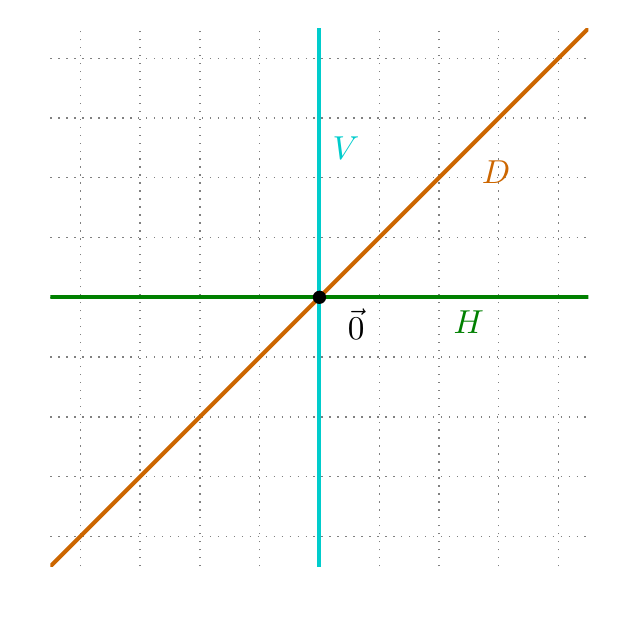
\begin{tikzpicture}[scale=1.2, >=latex]
    \begin{axis}[scale=1,
		    axis equal image,
		    axis line style={draw=none},
		    tick style={draw=none},
		    yticklabels={,,},
		    xticklabels={,,},
		 xmin=-4.5,
		 xmax=4.5,
		 ymin=-4.5,
		 ymax=4.5,
		 major grid style={dotted, gray},
                 xtick={-10,-9,...,10},
                 ytick={-10,-9,...,10},
                 grid=both,
		 anchor=origin]

	    \draw[Green, very thick] (-5,0) -- (5,0) node[near end, below] {$H$};
	    \draw[cyan!80!black, very thick] (0,-5) -- (0,5) node[near end, right] {$V$};
	    \draw[orange!80!black, very thick] (-5,-5) -- (5,5) node[near end, below right] {$D$};

	    \fill[fill=black] (0,0) circle[radius=2pt] node[below right, xshift=5pt] {\color{black}$\vec 0$};
    \end{axis}
\end{tikzpicture}
		\end{solution}
		\item $N=\Set*{\vec x\in\R^2 \given \vec x=t\mat{1\\1}\text{ for all }t\in\R}$.
				\begin{solution}[inline]
			$N=\Set{}$.
		\end{solution}

		\item $V\cup H$.
			\begin{solution}[inline]
			$V\cup H$ looks like a ``$+$'' going through the origin.
		\end{solution}
		\item $V\cap H$.
			\begin{solution}[inline]
				$V\cap H=\Set{\vec 0}$ is just the origin.
		\end{solution}
		\item Does $V\cup H=\R^2$?
			\begin{solution}
				No. $V\cup H$ does not contain $\mat{1\\1}$ while $\R^2$ does contain
				$\mat{1\\1}$.
			\end{solution}
	\end{parts}
\end{slide}


	\begin{bookonly}\begin{center}\hspace{-2cm}\triplegrid\hspace{-2cm}\triplegrid\end{center}\end{bookonly}
	\bookonlynewpage
	\displayonlynewpage
\section*{Vector Combinations}
	\vspace{-1em}

\begin{slide}
	\SavedDefinitionRender{LinearCombination}

	\question
	\label{ProbSkewBasis}
	\begin{annotation}
		\begin{goals}
			\Goal{Practice linear combinations.}

			The goal of this problem is to
			\begin{itemize}
				\item Practice using the formal term \emph{linear combination}.
				\item Foreshadow span.
			\end{itemize}
		\end{goals}

		\begin{notes}
			\begin{itemize}
				\item In 2, the question should arise: ``Is $3\vec v_1$
					a linear combination of $\vec v_1$ \emph{and}
					$\vec v_2$?'' Address this.
				\item Refer to the magic carpet ride for 5. You don't
					need to do a full proof.
			\end{itemize}
		\end{notes}
	\end{annotation}
	Let $\vec v_1=\mat{1\\1}$, $\vec v_2=\mat{1\\-1}$, and $\vec w=2\vec v_1+\vec v_2$.
	\begin{parts}
		\item Write $\vec w$ as a column vector. When $\vec w$ is written as a
			linear combination of $\vec v_1$ and $\vec v_2$, what are the
			coefficients of $\vec v_1$ and $\vec v_2$?
			\begin{solution}
				$\vec w=\mat{3\\1}$; the coefficients are $(2,1)$.
			\end{solution}
		\item Is $\mat{3\\3}$ a linear combination of $\vec v_1$ and $\vec v_2$?
			\begin{solution}[inline]
				Yes. $\mat{3\\3}=3\vec v_1+0\vec v_2$.
			\end{solution}

		\item Is $\mat{0\\0}$ a linear combination of $\vec v_1$ and $\vec v_2$?
			\begin{solution}[inline]
				Yes. $\vec 0=0\vec v_1+0\vec v_2$.
			\end{solution}
		\item Is $\mat{4\\0}$ a linear combination of $\vec v_1$ and $\vec v_2$?
			\begin{solution}[inline]
				Yes. $\mat{4\\0}=2\vec v_1+2\vec v_2$.
			\end{solution}
		\item Can you find a vector in $\R^2$ that isn't a linear combination of
		$\vec v_1$ and $\vec v_2$?
			\begin{solution}
				No. $\mat{1\\0}=\tfrac{1}{2}\vec v_1+\tfrac{1}{2}\vec v_2$ and
				$\mat{0\\1}=\tfrac{1}{2}\vec v_1-\tfrac{1}{2}\vec v_2$.
				Therefore
				\[
					\mat{a\\b}
					= a\mat{1\\0}+b\mat{0\\1}
					= a(\tfrac{1}{2}\vec v_1+\tfrac{1}{2}\vec v_2)
						+b(\tfrac{1}{2}\vec v_1-\tfrac{1}{2}\vec v_2)
					=(\tfrac{a+b}{2})\vec v_1+(\tfrac{a-b}{2})\vec v_2.
				\]
				Therefore any vector in $\R^2$ can be written as linear combinations
				of $\vec v_1$ and $\vec v_2$.
			\end{solution}
		\item Can you find a vector in $\R^2$ that isn't a linear combination of
			$\vec v_1$?
			\begin{solution}
				Yes. All linear combinations of $\vec v_1$ have equal $x$ and
				$y$ coordinates, therefore $\vec w=\mat{2\\1}$ is not a linear
				combination of $\vec v_1$.
			\end{solution}
	\end{parts}
\end{slide}

\begin{slide}
	\bookonlynewpage
	\question
	\begin{annotation}
		\begin{goals}
			\Goal{Practice formal writing.}
		\end{goals}

		\begin{notes}
			\begin{itemize}
				\item Make everyone \emph{write}. They will think
					they can do it, but they will find it hard if
					they try.
			\end{itemize}
		\end{notes}
	\end{annotation}
	Recall the \emph{Magic Carpet Ride} task where the hover board could
	travel in the direction $\vec h=\mat{3\\1}$ and the magic carpet could
	move in the direction $\vec m=\mat{1\\2}$.
	\begin{parts}
		\item Rephrase the sentence \emph{``Gauss can be reached using just the
			magic carpet and the hover board''} using formal mathematical
			language.
			\begin{solution}
				Gauss's location can be written as a linear combination of
				$\vec m$ and $\vec h$.
			\end{solution}
		\item Rephrase the sentence \emph{``There is nowhere Gauss can hide
			where he is inaccessible by magic carpet and hover board''} using
			formal mathematical language.
			\begin{solution}
				Every vector in $\R^2$ can be written as a linear combination
				of $\vec m$ and	$\vec h$.
			\end{solution}
		\item Rephrase the sentence \emph{``$\R^2$ is the set of all linear
			combinations of $\vec h$ and $\vec m$''} using formal mathematical
			language.
			\begin{solution}
				$\R^2=\Set{\vec v\given \vec v=t\vec m+s\vec h\text{ for some }t,s\in \R}$.
			\end{solution}
	\end{parts}
\end{slide}
\begin{slide}
	\question
	Hi
	\question
	There

\end{slide}

\end{document}
